\documentclass[12pt,oneside]{memoir}

\usepackage{nus-bcomp-fyp-ca-report}

\usepackage{lipsum}

\addbibresource{references.bib}

\definecolor{DarkBlue}{RGB}{0, 42, 97}
\hypersetup{
    colorlinks=true,    % Enables colored links
    linkcolor=black,    % Color of internal links
    citecolor=black,    % Color of citations
    urlcolor=DarkBlue   % Color of external links
}

\title{Benchmarking and Improving OCR System for Southeast Asian Languages}
\author{Qiu Jiasheng, Jason}
\department{Department of Computer Science}
\faculty{School of Computing}
\university{National University of Singapore}
\academicyear{2024/2025}
\projectid{H0792230}
\supervisor{A/P Min-Yen Kan}
\advisor{Tongyao Zhu}

\begin{document}
\frontmatter

\pagestyle{plain}

\makecover

\setcounter{page}{1}

\maketitle

\chapter{Abstract}
While Optical Character Recognition (OCR) has been widely studied for high-resource languages such as English and Chinese, the efficacy and limitations of OCR models on Southeast Asian (SEA) languages remain largely unexplored.
This study aims to bridge this gap by assessing and improving the performance of OCR technologies on SEA languages.
To achieve this objective, we propose a reusable pipeline to gather SEA-language text from Wikipedia and benchmark popular OCR tools.

\vspace{20pt}
Subject Descriptors:
\begin{adjustwidth}{0.7in}{}
    I.2.7 Natural Language Processing
\end{adjustwidth}

Keywords:
\begin{adjustwidth}{0.7in}{}
    Optical Character Recognition, Southeast Asian Languages
\end{adjustwidth}

Implementation Software and Hardware:
\begin{adjustwidth}{0.7in}{}
    Python, Tesseract, EasyOCR
\end{adjustwidth}

\chapter{Acknowledgement}
I would like to thank my supervisor, A/P Kan Min-Yen, and my advisor, Tongyao Zhu, for their invaluable guidance and mentorship. Their encouragement and constructive guidance have been a significant source of inspiration throughout the project.

\listoffigures
\listoftables
\tableofcontents

\mainmatter

\chapter{Introduction}
Current research in Natural Language Processing (NLP) is heavily concentrated on 20 of the 7,000 languages in the world \parencite{magueresse-etal-2020}.
In particular, Southeast Asia (SEA) is home to over 1,000 languages but remains a relatively under-researched region in NLP \parencite{aji-etal-2023}.
Similar to most low-resource languages, a major challenge in developing NLP systems for SEA languages is the limited availability of datasets for the region’s languages.
Although many scanned documents and books in these low-resource languages are available online, the text within these files remains inaccessible due to formats like images and PDFs.

A solution to this problem is to use Optical Character Recognition (OCR) to extract the textual data.
OCR is the process of identifying and converting text in an image into a computer-friendly text format.
By extracting the text from these scanned documents, OCR can generate valuable datasets for low-resource languages.
The created datasets can then be used for downstream NLP tasks, such as machine translation, training large language models, and POS taggers \parencite{agarwal-and-anastasopoulos-2024, ignat-etal-2022}.
Therefore, studying OCR performance on SEA languages is crucial to accelerating NLP research in the region.

While OCR has been widely studied for high-resource languages such as English and Chinese, the efficacy and limitations of OCR models on SEA languages remain largely unexplored.
To address this gap, we propose a reusable pipeline to collect textual data in low-resource SEA languages from Wikipedia and benchmark popular open-source OCR tools on the collected data.
The primary objective is to benchmark and improve the performance of OCR technologies on SEA languages, thereby contributing to the advancement of NLP applications in this linguistically diverse region.
Specifically, this project seeks to answer the following research questions (RQs):

\begin{itemize}
    \item \textbf{RQ1.} How do popular OCR tools perform on SEA scripts?
    \item \textbf{RQ2.} What specific linguistic and script-related challenges affect OCR accuracy on SEA languages?
    \item \textbf{RQ3.} What techniques and recommendations can enhance OCR accuracy on SEA languages?
\end{itemize}

\chapter{Related Work}

Several studies have been done to benchmark OCR performance on low-resource languages.
They follow a similar methodology of collecting data in several languages, followed by an evaluation of a chosen set of OCR tools.

\section{Collecting Low-Resource Language Data}
To evaluate OCR performance accurately, a collection of textual data in the form of images or PDFs paired with reliable ground truth is essential.
Similar to most NLP tasks, data scarcity poses a major obstacle to advancing OCR technology in low-resource languages, where the limited availability of annotated textual data restricts both model training and evaluation.
Although an abundance of scanned documents in these low-resource languages exists online, they lack the ground truth required for evaluation.
While plain text in these languages is often available separately, it typically exists in text-based formats rather than images or PDFs, limiting its direct usefulness as ground truth for OCR.

To bridge this gap, many studies rely on artificial images and PDFs generated from plain text to create usable evaluation data.
\textcite{hegghammer-2022} sourced Arabic data from the Yarmouk Arabic OCR Dataset, a collection of 4,587 Wikipedia articles printed out and scanned back to PDF, paired with ground truth in TXT files.
\textcite{ignat-etal-2022} artificially created PDFs from the Flores 101 dataset, which consists of text data from Wikipedia in 101 languages.
Generalizing this concept of a document creation pipeline further, \textcite{gupte-etal-2021} published an open-source Python package for generating document images from plain text, including several document styling templates.
Using these methods, high-quality low-resource language data paired with ground truth can be generated from text-based formats on a large scale.

A common trend in using artificial data is the augmentation of noise to simulate real-world conditions, which often contain complex layouts, stains, and scribbles \parencite{hegghammer-2022}.
Directly using noise-free data, i.e., single-column text in a clear font, limits OCR processors' usefulness on real-life scanned documents.
Thus, noise augmentation is often applied to artificial data.
Some popular techniques include changing font style, size, color, letter spacing, and adding Gaussian blur, bleed-through, and salt-and-pepper noise \parencite{gupte-etal-2021, ignat-etal-2022}.

\section{Existing OCR Systems}
To benchmark OCR performance programmatically, there are two broad categories of OCR systems: open-source and commercial.

Open-source OCR systems are characterized by their accessibility, allowing users to view, modify, and distribute the source code freely.
This transparency enables developers to customize the tools to meet specific needs.
Furthermore, open-source systems typically incur no licensing fees, making them cost-effective options for research purposes.
For instance, Tesseract \parencite{smith-2013}, regarded as one of the most accurate open-source OCR engines, consistently maintains its popularity in the research community \parencite{hegghammer-2022, ignat-etal-2022}.

Commercial OCR systems are typically accessed through paid services via application programming interfaces (APIs).
Notable examples of these systems include Amazon Textract, Google Document AI, and Google Vision API.
Generally, commercial off-the-shelf OCR tools tend to perform better than their open-source counterparts \parencite{hegghammer-2022, ignat-etal-2022}.
However, the proprietary nature of these "black box" models limits their utility for research purposes, such as fine-tuning and customization.
Additionally, the associated costs of these services contribute to fewer studies focused on commercial systems in comparison to the more widely researched open-source tools.

\begin{table}[ht]
    \centering
    \begin{tabular}{lllll}
        \toprule
        & Category & Provider & Languages & Cost\\
        \midrule
        Tesseract & Open-source & - & 116 & Free\\
        EasyOCR & Open-source & Jaided AI & 83 & Free\\
        Textract & Commercial & Amazon & 6 & \$1.50 per 1000 pages \\
        Document AI & Commercial & Google & 6 & \$1.50 per 1000 pages\\
        Vision API & Commercial & Google & 6 & \$1.50 per 1000 pages\\
        \bottomrule
    \end{tabular}
    \caption{Summary of popular open-source and commercial OCR processors}
   \label{table:summary-of-ocr-processors}
\end{table}

\section{Benchmarking OCR}
Applying OCR yields a plain text prediction, which is then compared with the ground truth data to assess the tool’s accuracy and performance.
Recent studies have demonstrated that OCR systems tend to perform better on artificially generated data than on real-world data \parencite{ignat-etal-2022}.
This observation suggests that synthetic datasets may not fully capture the complexities of authentic documents, which often feature issues like imperfect text alignment, varied fonts, and complex layouts.
Furthermore, the addition of synthetic noise significantly raises error rates, especially for open-source systems, which appear more susceptible to noise interference than their commercial counterparts \parencite{hegghammer-2022}.

\textcite{ignat-etal-2022} also show that OCR tools generally achieve higher accuracy on scripts written in Latin alphabets.
This disparity in performance partly stems from market incentives that prioritize the development of English-language OCR systems, resulting in more extensive training data and refinement for Latin-based scripts \parencite{hegghammer-2022}. 
Ornate scripts, such as those with complex diacritics or unique letter shapes, present additional challenges and tend to yield lower OCR accuracy.
Although \textcite{hegghammer-2022} focuses on English and Arabic, techniques from similar studies on non-SEA languages offer valuable insights for creating SEA-specific OCR benchmarks.

In terms of benchmarking OCR on SEA languages, the most related study is the recent work by \textcite{ignat-etal-2022}.
They grouped 60 low-resource languages by region and script, including SEA languages like Khmer, Lao, Burmese, Thai, and Vietnamese.
Their research revealed that while OCR models perform well on artificial SEA-language data, accuracy drops significantly on real-world data.
This discrepancy underscores the need for more real-world training data to improve OCR outcomes for SEA languages.

In summary, there exists a gap in benchmarking OCR specifically for SEA languages, largely due to the lack of real-world training data.
This project addresses this gap by proposing a reusable pipeline for benchmarking OCR performance on real-world SEA-language data sourced from Wikipedia.

\chapter{Methodology}

\section{Data Selection}

\subsection{Source of Data}
We chose to use Wikipedia as our text corpus for several reasons.
Firstly, Wikipedia articles can be easily converted into images via screenshots, making them suitable for OCR applications. 
The platform also offers a convenient source of ground truth through its APIs that provide plain text for most articles, facilitating accurate evaluation. 
Secondly, Wikipedia hosts a large corpus in several popular SEA languages, including Thai, Vietnamese, Indonesian, Tamil, and Burmese, supporting our language needs \parencite{list-of-wikipedias-2024}. 
Lastly, Wikipedia articles share a consistent format and layout across languages, which is representative of real-world data. 
This uniform structure helps to eliminate a variable in our study, allowing us to focus on assessing the performance of OCR.

\subsection{Languages}
From the languages available on Wikipedia, we selected English, Indonesian, Vietnamese, and Thai text. 
English serves as a baseline for sanity checks and bug fixing, given our familiarity with the language. 
The remaining SEA languages were chosen to capture diverse script characteristics. 
Indonesian represents Latin-based scripts, Vietnamese represents Latin scripts with diacritics, and Thai represents non-Latin scripts. 

\subsection{Dataset}
We compiled a dataset of 100 Wikipedia articles, selecting the 20 most viewed English articles 
from each of five categories: people, present countries, cities\footnote{Singapore was replaced 
because it's already listed under present countries.}, life, and buildings and structures\footnote{Machu 
Picchu was replaced because it's already listed under cities.} 
\parencite{wikipedia-popular-pages-2024}.
These categories were chosen to create a diverse corpus in terms of content. 
We prioritized high-view articles because they are more likely to have substantial data available across languages. 
Table \ref{table:dataset} lists the articles included in our dataset.

\section{Data Collection}

\begin{figure}[ht]
    \centering
    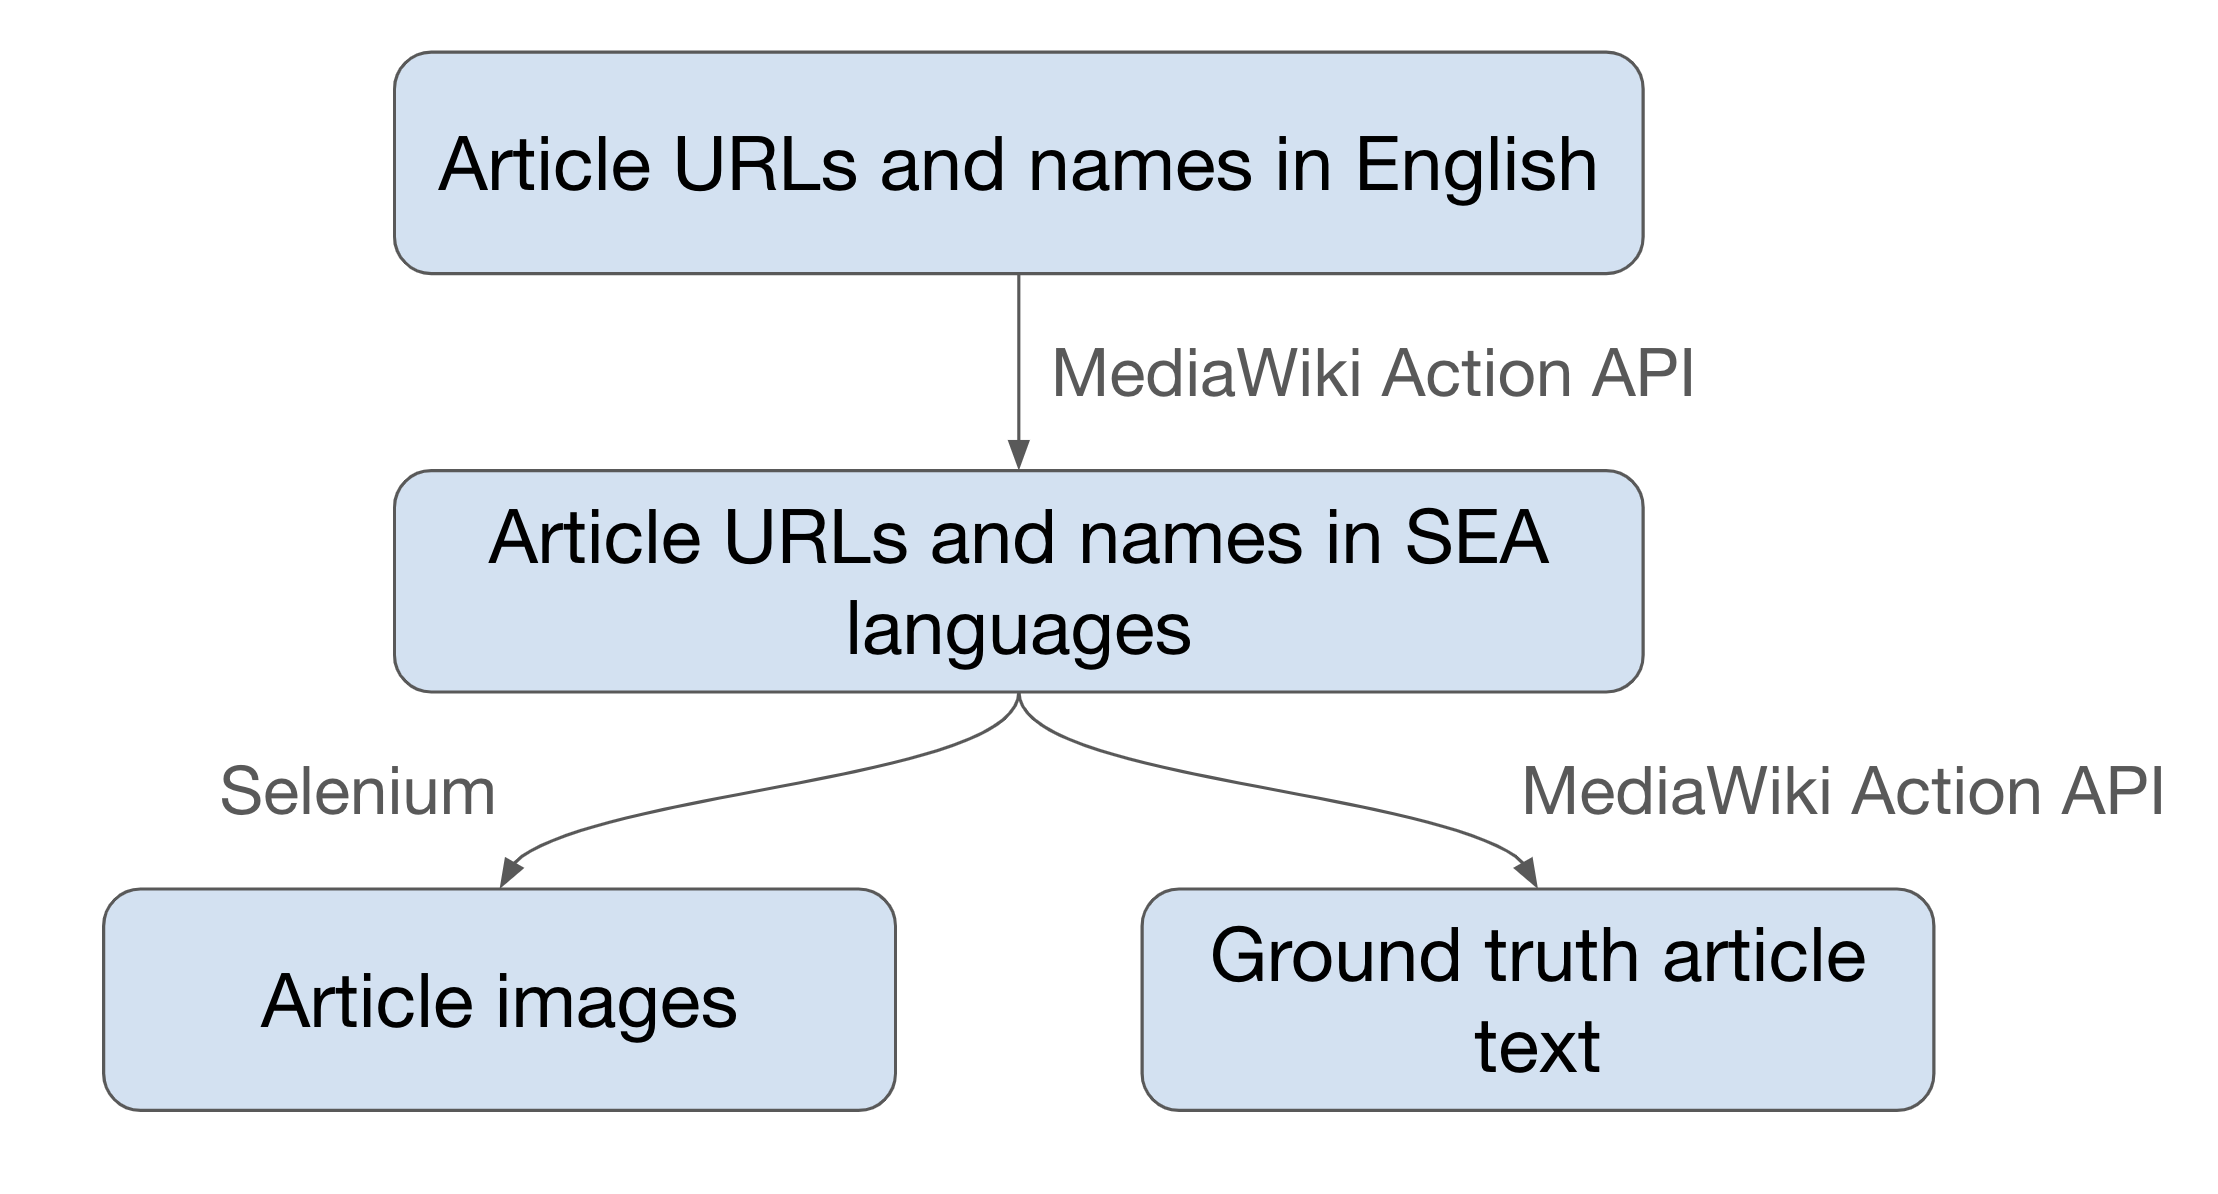
\includegraphics[width=0.6\textwidth]{images/data-collection.png}
    \caption{Pipeline for data collection from Wikipedia}
    \label{figure:data-collection}
\end{figure}

From the dataset of 100 Wikipedia articles, we collected article images and ground 
truth article text in our selected languages using Python, 
Selenium\footnote{\href{https://selenium-python.readthedocs.io}{Selenium} is a 
framework for automating web browsers, commonly used for web scraping by programmatically 
interacting with websites.}, and the MediaWiki Action API\footnote{The \href{https://www.mediawiki.org/wiki/API:Main_page}{MediaWiki Action API} allows 
access to wiki page operation features such as search and retrieval.}. Figure \ref{figure:data-collection} illustrates the overall pipeline 
for data collection. The detailed steps are as follows:

\begin{enumerate}
    \item Manually compile the dataset’s article names and URLs in English.
    \item Fetch the article names and URLs in Thai, Vietnamese, and Indonesian from the MediaWiki Action API.
    \item Download the articles in all languages in PDF format using Selenium.
    \item Convert the article PDFs into PNG images. Each image represents one page in the PDF.
    \item Download the ground truth article text into TXT files from the MediaWiki Action API.
\end{enumerate}

\section{OCR Evaluation}

\subsection{OCR Systems}
In our selection of OCR systems for benchmarking, we prioritized open-source 
solutions that support a diverse range of SEA languages, as this approach 
enhances accessibility and encourages collaboration within the research community. 
Consequently, we selected to use Tesseract and EasyOCR. 

Tesseract\footnote{\url{https://github.com/tesseract-ocr/tesseract}} is an established OCR engine, recognized as one of the top performers 
in the 1995 UNLV Test \parencite{rice-etal-1995}. It utilizes an underlying Long Short-Term Memory (LSTM) 
model. EasyOCR\footnote{\url{https://github.com/JaidedAI/EasyOCR}} is a modern OCR framework that integrates a text detection model 
based on the Character Region Awareness for Text (CRAFT) algorithm with a 
recognition model utilizing a Convolutional Recurrent Neural Network (CRNN). Both 
Tesseract and EasyOCR provide robust support for English, Indonesian, Vietnamese, 
and Thai, making them suitable candidates for our benchmarking study.

\subsection{Evaluation Metrics}

\begin{equation}
    CER = \frac{I + D + S}{N}
    \label{equation:cer}
\end{equation}

Similar to most OCR benchmark studies, we utilize Character Error Rate (CER) and 
Word Error Rate (WER) as our evaluation metrics \parencite{hegghammer-2022, ignat-etal-2022}. CER measures the accuracy of 
character recognition and is calculated using the Levenshtein or edit distance, 
which represents the minimum number of single-character insertions (I), deletions (D), 
and substitutions (S) required to transform one word into another. As shown in 
Equation \ref{equation:cer}, CER is defined as the edit distance between the 
OCR-predicted text and ground truth text, divided by the total number of characters 
in the ground truth text (N). A lower CER value indicates higher accuracy, with 
0 representing perfect recognition. Notably, CER can exceed 1, particularly when 
there are a significant number of insertions. WER serves as the word-based counterpart to CER.

\subsection{Data Validation and Cleaning}
The raw predicted text generated by the OCR tools exhibited extremely high error 
rates. Upon further investigation, we identified some consistent formatting issues 
in the output:

\begin{itemize}
    \item Tesseract adds an additional space character after every predicted character, leading to CERs exceeding 1.
    \item The article images included references and in-text citations, which are not present in the ground truth. 
\end{itemize}

To address these issues, we performed data cleaning to align the output text 
more closely with the ground truth. This cleaning significantly reduced the error 
rates to more acceptable levels.

We then implemented a data validation step to automatically check the CERs for 
each language. Articles were flagged as outliers if the CER between the OCR-predicted 
text and the ground truth text exceeded two standard deviations from the mean \parencite{cousineau-and-chartier-2010}. 
We manually reviewed these outlier articles for anomalies, resulting in the removal 
of seven articles where the images and ground truth texts contained different content.

\subsection{Summary}

\begin{figure}[ht]
    \centering
    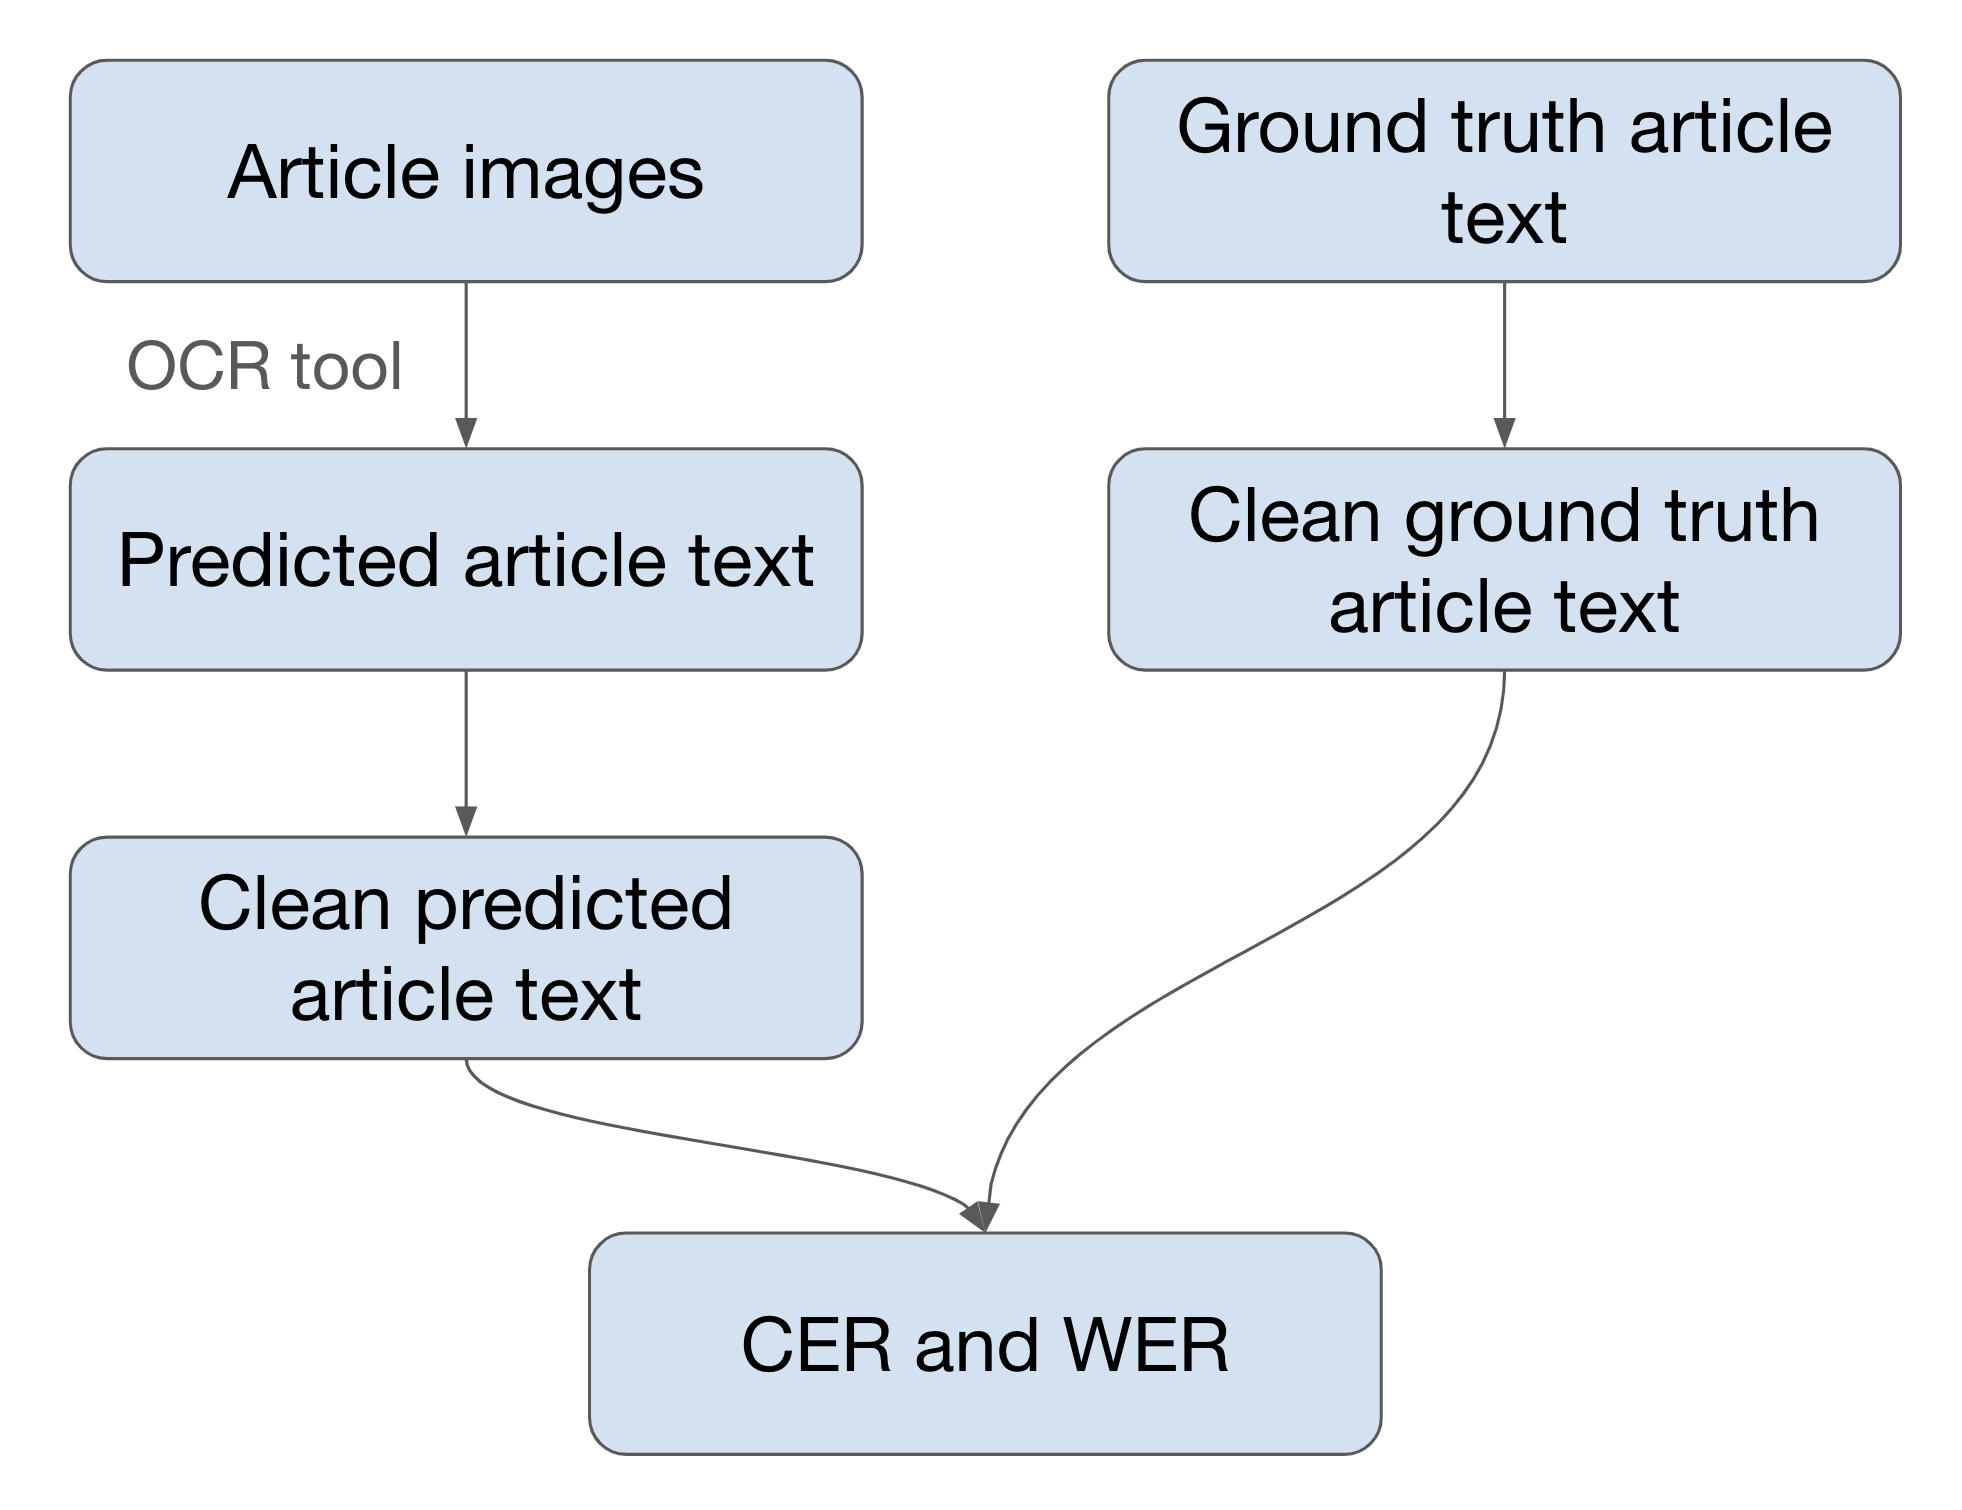
\includegraphics[width=0.6\textwidth]{images/ocr-evaluation.png}
    \caption{Pipeline for OCR evaluation}
    \label{figure:ocr-evaluation}
\end{figure}

In summary, we evaluated the CER and WER for each article using the images and 
ground truth text collected from our data pipeline. Figure \ref{figure:ocr-evaluation} 
illustrates the overall pipeline for OCR evaluation. The detailed steps are as follows:

\begin{enumerate}
    \item Apply the OCR tools on the article images.
    \item Perform data cleaning on the predicted article text and ground truth article text.
    \item Compute the CER and WER between the predicted text and the ground truth text using JiWER\footnote{\href{https://pypi.org/project/jiwer/}{JiWER} is a Python package designed for fast calculation of CER and WER.}.
\end{enumerate}

\chapter{Results}

\begin{table}[ht]
    \centering
    \begin{tabular}{lcccc}
        \toprule
        & \multicolumn{2}{c}{\textbf{Character Error Rate}} & \multicolumn{2}{c}{\textbf{Word Error Rate}}\\
        \cmidrule(lr){2-3}\cmidrule(lr){4-5}
        & EasyOCR & Tesseract & EasyOCR & Tesseract\\
        \midrule
        English & 0.17 & 0.20 & 0.25 & 0.29\\
        Indonesian & 0.20 & 0.18 & 0.27 & 0.33\\
        Vietnamese & 0.30 & 0.39 & 0.31 & 0.42\\
        Thai & 0.26 & 0.51 & 1.68 & 1.77\\
        \bottomrule
    \end{tabular}
    \caption{Average Character Error Rate and Word Error Rate}
    \label{table:results}
\end{table}

Table \ref{table:results} presents the average CER and WER for each language and 
OCR model. The results reveal several key observations on the performance of popular OCR tools on SEA languages(\textbf{RQ1}):

\begin{itemize}
    \item EasyOCR generally outperforms Tesseract, yielding lower error rates.
    \item Both OCR tools perform best on Latin scripts (English and Indonesian), followed by Latin scripts with diacritics (Vietnamese), and then Non-Latin scripts (Thai).
    \item The WER for Thai is notably high due to its non-segmented script structure.
\end{itemize}

\section{Discussion}
There is no universal standard for what makes a “good” CER or WER value, as OCR 
performance varies widely depending on factors like text complexity, layout, and 
print quality. While many OCR systems claim accuracy rates of 99\%, \textcite{holley-2009} argues 
that these rates typically apply to clean images or to cases with manual 
intervention during the OCR process. Supporting this claim, \textcite{hegghammer-2022} found that his 
WER on English articles averaged around 0.01 (nearly perfect) on clean images 
but surged to a WER of 0.22 when noise was introduced. For comparison, our 
average WER on English articles is 0.27. Therefore, our results align with 
similar studies that benchmark OCR on noisy, real-world data. 

\begin{figure}[ht]
    \centering
    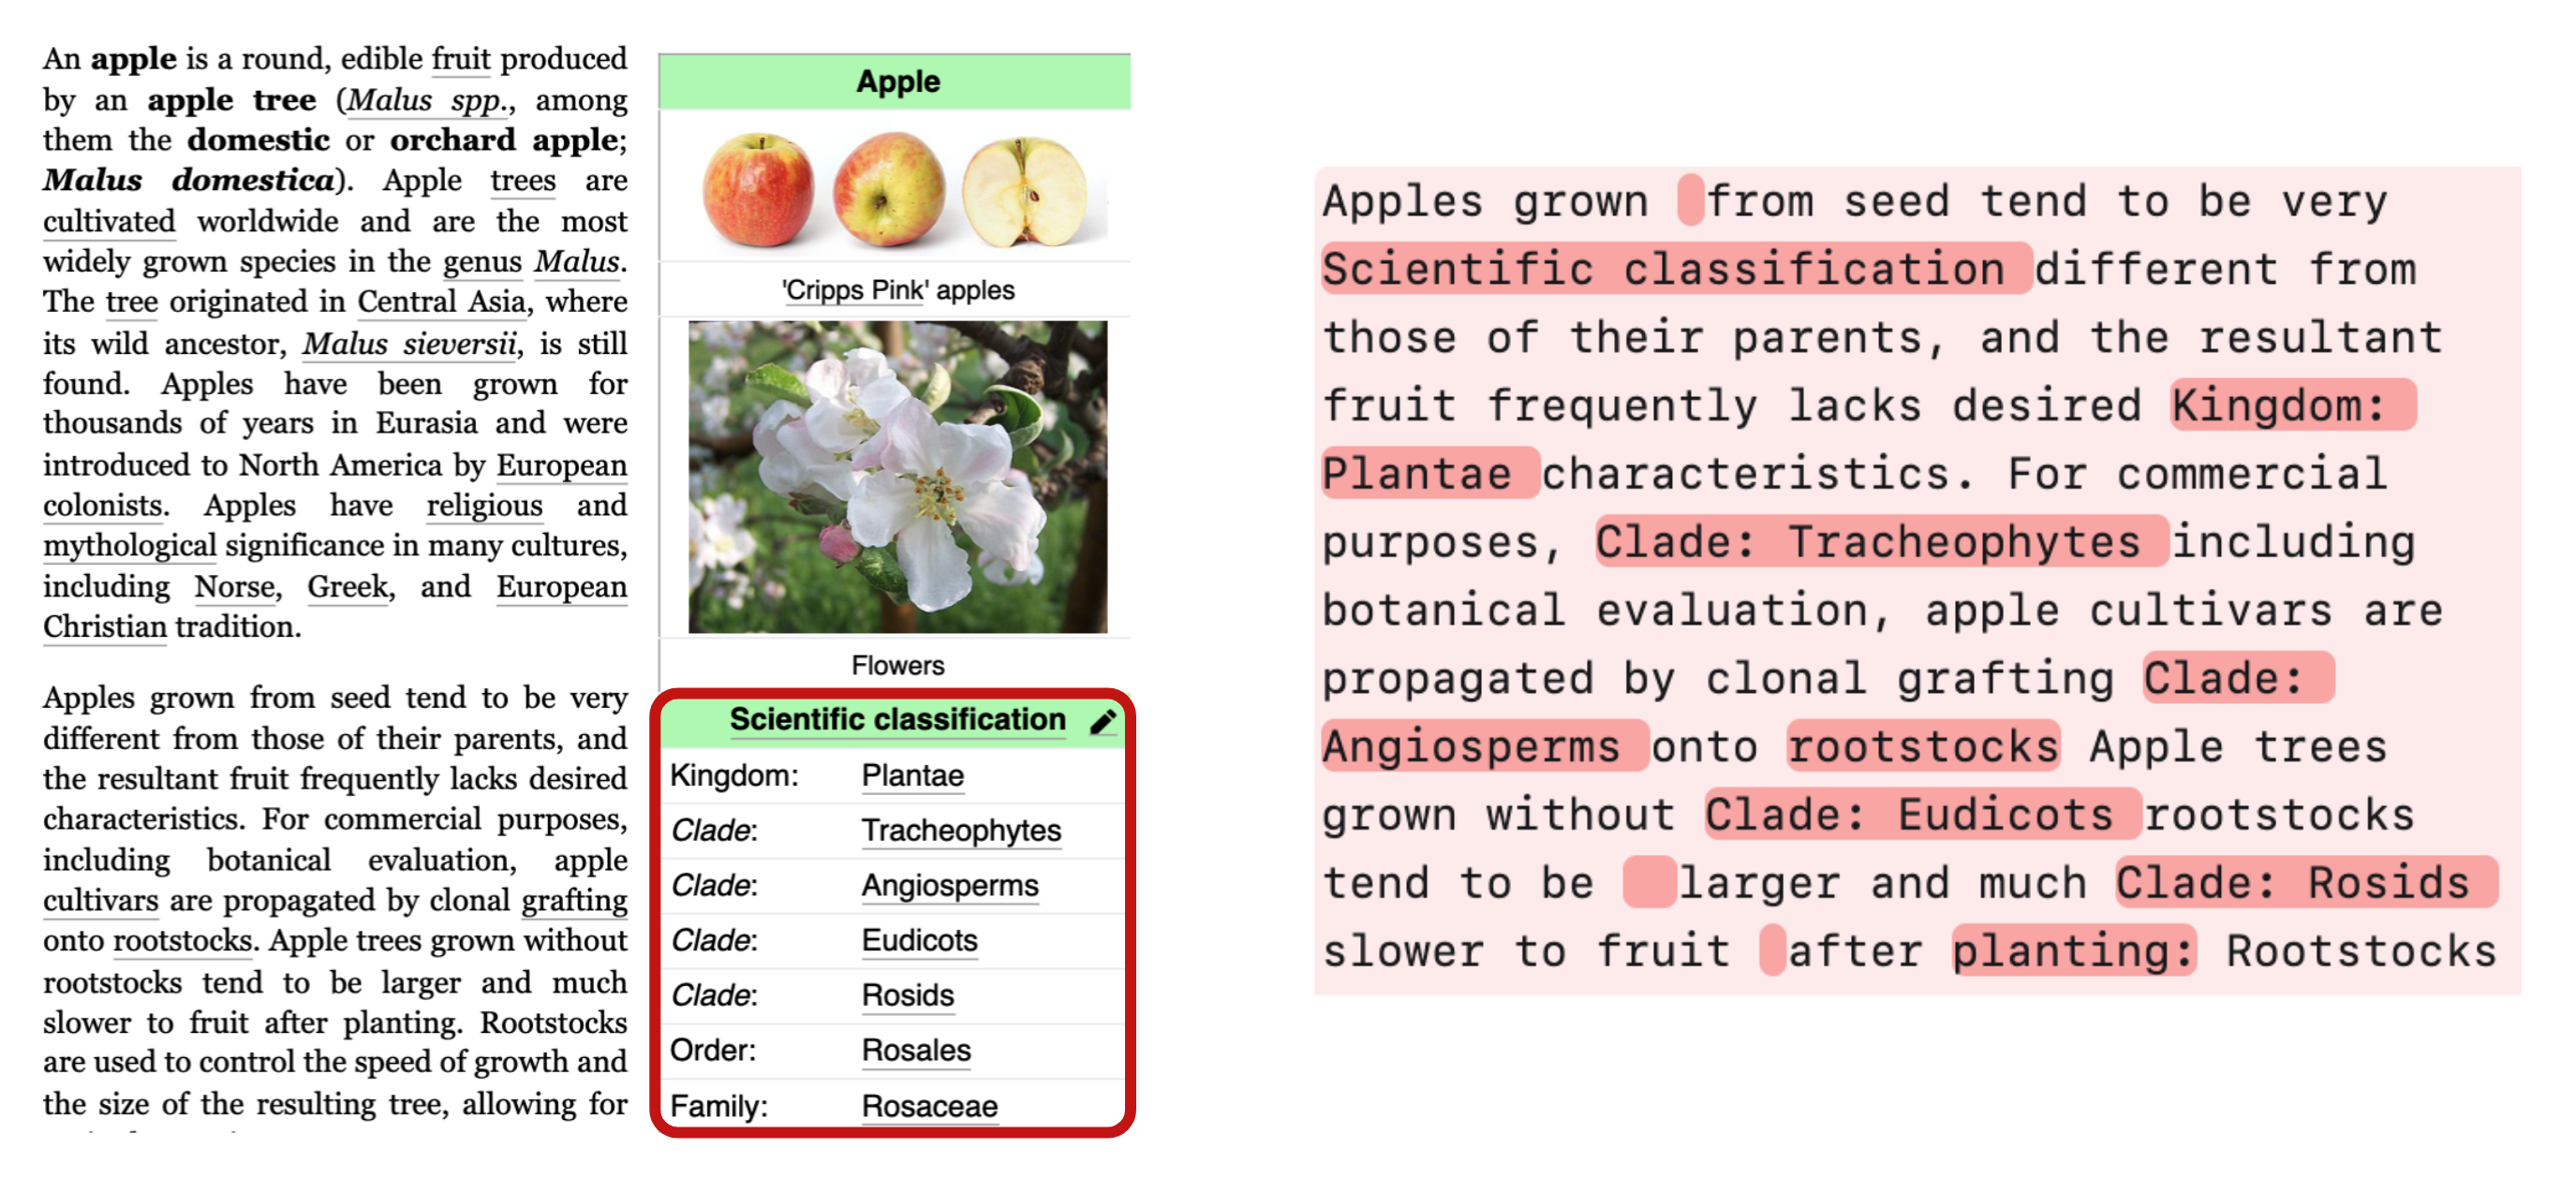
\includegraphics[width=0.9\textwidth]{images/multimodal-content.png}
    \caption{OCR systems detect extraneous elements as additional text}
    \label{figure:multimodal-content}
\end{figure}

Manual comparison of the OCR-predicted text and the ground truth reveals that most 
errors arise from Wikipedia’s complex layout and multimodal content, such as 
tables and embedded text within images. As shown in Figure \ref{figure:multimodal-content}, 
OCR tools often detect these elements as additional text, which is absent from 
the ground truth, leading to discrepancies. This issue highlights the challenge 
OCR systems face with multimodal formats, where extraneous elements are 
misinterpreted as part of the textual content.

\chapter{Future Work}
In summary, this study examines the performance of OCR systems on SEA languages. 
We developed a reusable pipeline for collecting real-world data from Wikipedia 
to generate images and ground truth text from 100 articles in English, 
Indonesian, Vietnamese, and Thai. Using this dataset, we benchmarked Tesseract 
and EasyOCR, yielding results comparable to those in recent studies.

For future studies, we hope to focus on the following:

\begin{itemize}
    \item Expand our text corpus to other SEA languages.
    \item Try other more OCR tools (e.g., transformer-based)
    \item Identify language-specific challenges faced by OCR in the results (RQ2).
    \item Suggest techniques and recommendations to enhance OCR accuracy on SEA languages (RQ3).
\end{itemize}

\printbibliography[title={References}]

\clearpage
\appendix
\renewcommand{\chaptername}{Appendix}

\chapter{Wikipedia Article Dataset}

\begin{table}[ht]
    \centering
    \begin{tabular}{p{1in}p{3.8in}}
        \toprule
        \textbf{Category} & \textbf{Articles} \\
        \midrule
        People & Donald Trump, Elizabeth II, Barack Obama, Christiano Ronaldo, Michael Jackson, Elon Musk, Lady Gaga, Adolf Hitler, Eminem, Lionel Messi, Justin Bieber, Freddie Mercury, Kim Kardashian, Johnny Depp, Steve Jobs, Dwayne Johnson, Michael Jordan, Taylor Swift, Stephen Hawking, Kanye West\\
        \midrule
        Present countries & United States, India, United Kingdom, Canada, Australia, China, Russia, Japan, Germany, France, Singapore, Israel, Pakistan, Philippines, Brazil, Italy, Netherlands, New Zealand, Ukraine, Spain\\
        \midrule
        Cities & New York City, London, Hong Kong, Los Angeles, Dubai, Washington, D.C., Paris, Chicago, Angelsberg, Mumbai, San Francisco, Rome, Monaco, Toronto, Tokyo, Philadelphia, Machu Picchu, Jerusalem, Amsterdam, Boston\\
        \midrule
        Life & Cat, Dog, Animal, Lion, Coronavirus, Tiger, Human, Dinosaur, Elephant, Virus, Horse, Photosynthesis, Evolution, Apple, Bird, Mammal, Potato, Polar bear, Shark, Snake\\
        \midrule
        Buildings and structures & Taj Mahal, Burj Khalifa, Statue of Liberty, Great Wall of China, Eiffel Tower, Berlin Wall, Stonehenge, Mount Rushmore, Colosseum, Auschwitz concentration camp, Great Pyramid of Giza, One World Trade Center, Empire State Building, White House, Petra, Large Hadron Collider, Hagia Sophia, Golden Gate Bridge, Panama Canal, Angkor Wat\\
        \bottomrule
    \end{tabular}
    \caption{Dataset of 100 Wikipedia articles}
    \label{table:dataset}
\end{table}

\end{document}
